\documentclass[11pt, a4paper]{article}
\usepackage[utf8]{inputenc}
\usepackage[T1]{fontenc}
\usepackage{geometry}
\usepackage{subcaption}
\usepackage{graphicx}
\usepackage{float}
\geometry{a4paper, top=2.5cm, bottom=2.5cm, left=2.5cm, right=2.5cm}
\usepackage{multirow}
\usepackage{tabularx}
\usepackage{array}
\usepackage{booktabs}
\usepackage{placeins}

\usepackage{tikz}
\usetikzlibrary{calc} 
\usetikzlibrary{arrows.meta, positioning}
\usepackage{url}
\usepackage[hidelinks]{hyperref}

\usepackage{amsmath}
\usepackage{amssymb} 

\usepackage{fancyhdr}
\pagestyle{fancy}
\fancyhf{}                 % clear header/footer
\fancyfoot[C]{\thepage}    % page number center footer

% --- ONLY section updates the header ---
\renewcommand{\sectionmark}[1]{%
    \markright{\thesection\ #1}
}

% --- disable subsection from touching the header ---
\renewcommand{\subsectionmark}[1]{}

% --- header layout ---
\fancyhead[L]{GROUP 1} 
\fancyhead[R]{\rightmark}
\makeatletter
\renewcommand{\@seccntformat}[1]{\csname the#1\endcsname.\quad}
\makeatother
\setlength{\parindent}{0pt}
\setlength{\parskip}{6pt}
\usepackage{adjustbox}

\begin{document}

% ======================= COVER PAGE ==========================
\thispagestyle{empty}

% Draw the border frame
\begin{tikzpicture}[remember picture, overlay]
  \draw[line width=0.8pt]
  ($(current page.north west) + (2cm,-2cm)$)
  rectangle
  ($(current page.south east) + (-2cm,2cm)$);
\end{tikzpicture}

\begin{center}

  {\large \textbf{UNIVERSITY OF SCIENCE AND TECHNOLOGY OF HANOI}}\\[4pt]
  {\normalsize \textbf{DEPARTMENT OF INFORMATION AND COMMUNICATION TECHNOLOGY}}\\[3cm]

  \includegraphics[width=6cm]{images/logo.png}\\[2cm]

  {\LARGE \textbf{INTRODUCTION TO CRYPTOGRAPHY MIDTERM PROJECTS}}\\[0.5cm]
  {\large \textbf{Group 1}}\\[0.5cm]
  {\Large \textbf{RSA Digital Signatures for Data Integrity}}\\[2cm]

  {\large \textit{Members:}}\\[4pt]
  {\large
  Trinh Nhat Huy - 23BI14193\\
  Nguyen Minh Tuan - 23BI14441\\
  Nguyen Quang Minh - 23BI14288\\
  Hoang Quang Minh - 23BI14281}\\
  Le Huy Hoang - 23BI14172\\[1cm]

  {\large Hanoi, \today}

\end{center}

% ======================= FRONTMATTER ==========================
\newpage
% Dùng số La Mã cho các trang râu ria
\tableofcontents
\thispagestyle{empty}
% List of figures removed to save space (only 2 figures)

% ======================= MAIN CONTENT ==========================
\newpage
\pagenumbering{arabic} % Bắt đầu đếm trang 1, 2, 3... cho phần nội dung chính
\setcounter{page}{1}

% Gọi các file con từ thư mục sections/
\section{Introduction}

In modern digital communication, data is constantly transmitted over public, insecure networks, making it vulnerable to interception, tampering, and forgery. Cryptography provides the fundamental tools to address these threats—not only through encryption, but also through mechanisms that guarantee \textbf{authenticity} and \textbf{integrity} of information.

A \textbf{digital signature} is the mathematical equivalent of a handwritten signature: it binds the identity of a signer to the content of a message, ensuring that any modification after signing is immediately detectable. The RSA algorithm (Rivest–Shamir–Adleman), one of the most widely adopted asymmetric cryptosystems, serves as the foundation for this project.

This report explores both the theory and practice of RSA digital signatures. It covers the mathematical foundations (key generation, modular arithmetic), presents the system architecture and a working Python implementation, analyzes security properties, and evaluates performance across different hash algorithms.
\section{Mathematical Foundation}

\subsection{Key Generation}
The RSA key pair consists of a public key $(e, n)$ and a private key $(d, n)$, generated as follows:

\textbf{Step 1.} Select two distinct large primes $p$ and $q$, verified using the \textbf{Miller-Rabin} primality test.

\textbf{Step 2.} Compute the modulus: $n = p \times q$.

\textbf{Step 3.} Compute Euler's totient: $\phi(n) = (p-1)(q-1)$.

\textbf{Step 4.} Choose public exponent $e$ such that $1 < e < \phi(n)$ and $\gcd(e, \phi(n)) = 1$. The standard choice is $e = 65537$.

\textbf{Step 5.} Compute private exponent $d = e^{-1} \bmod \phi(n)$ using the Extended Euclidean Algorithm:
$$ e \times d \equiv 1 \pmod{\phi(n)} $$

\subsection{Signing and Verification}
Let $H$ be the integer representation of the hash of the message, reduced modulo $n$.

\textbf{Signing} (private key): The signer computes the signature $S$:
$$ S \equiv H^d \pmod{n} $$

\textbf{Verification} (public key): The verifier recovers the hash:
$$ H' \equiv S^e \pmod{n} $$

By Euler's theorem, since $e \cdot d \equiv 1 \pmod{\phi(n)}$:
$$ S^e \equiv (H^d)^e \equiv H^{ed} \equiv H \pmod{n} $$
If $H' = H$, the signature is valid—proving both \textbf{authenticity} and \textbf{data integrity}.

\section{System Architecture}

The RSA digital signature system follows a linear pipeline divided into four stages. Figure~\ref{fig:flowchart} illustrates the complete signing and verification workflow.

\begin{figure}[H]
    \centering
    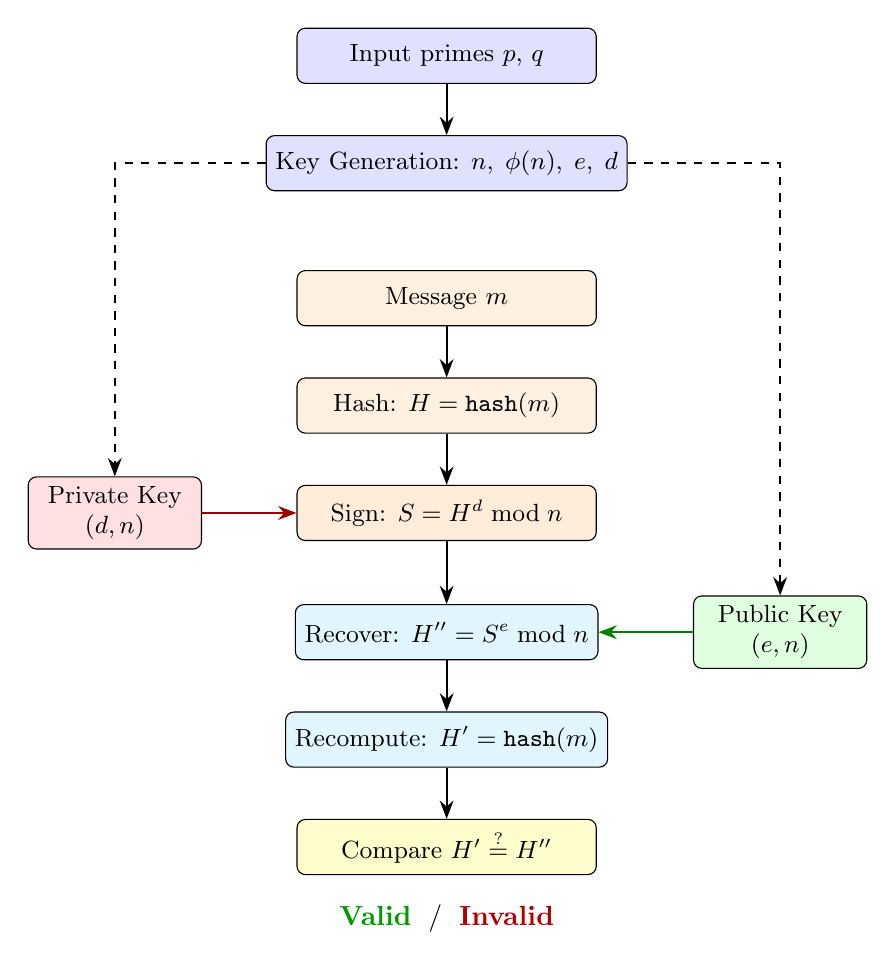
\begin{tikzpicture}[
            node distance=0.65cm,
            box/.style={rectangle, draw, rounded corners=3pt, minimum width=3.8cm, minimum height=0.7cm, align=center, font=\small},
            key/.style={rectangle, draw, rounded corners=3pt, minimum width=2.2cm, minimum height=0.6cm, align=center, font=\small},
            arrow/.style={-Stealth, thick}
        ]

        % Stage 1: Key Generation
        \node[box, fill=blue!12] (primes) {Input primes $p$, $q$};
        \node[box, fill=blue!12, below=of primes] (keygen) {Key Generation: $n,\;\phi(n),\;e,\;d$};
        \draw[arrow] (primes) -- (keygen);

        % Stage 2: Hashing
        \node[box, fill=orange!12, below=1.0cm of keygen] (msg) {Message $m$};
        \node[box, fill=orange!12, below=of msg] (hash) {Hash: $H = \texttt{hash}(m)$};
        \draw[arrow] (msg) -- (hash);

        % Stage 3: Signing
        \node[box, fill=orange!15, below=of hash] (sign) {Sign: $S = H^d \bmod n$};
        \node[key, fill=red!12, left=1.2cm of sign] (privkey) {Private Key\\$(d, n)$};
        \draw[arrow] (hash) -- (sign);
        \draw[arrow, color=red!60!black] (privkey) -- (sign);

        % Stage 4: Verification
        \node[box, fill=cyan!12, below=0.8cm of sign] (recover) {Recover: $H'' = S^e \bmod n$};
        \node[key, fill=green!12, right=1.2cm of recover] (pubkey) {Public Key\\$(e, n)$};
        \node[box, fill=cyan!12, below=of recover] (rehash) {Recompute: $H' = \texttt{hash}(m)$};
        \node[box, fill=yellow!20, below=of rehash] (compare) {Compare $H' \stackrel{?}{=} H''$};
        \draw[arrow] (sign) -- (recover);
        \draw[arrow, color=green!50!black] (pubkey) -- (recover);
        \draw[arrow] (recover) -- (rehash);
        \draw[arrow] (rehash) -- (compare);

        % Dashed lines from Key Generation to both keys
        \draw[arrow, dashed] (keygen.west) -| (privkey.north);
        \draw[arrow, dashed] (keygen.east) -| (pubkey.north);

        % Result — two colors matching the diagram
        \node[below=0.25cm of compare] {%
            \textbf{\color{green!60!black}Valid} \;/\; \textbf{\color{red!70!black}Invalid}%
        };

    \end{tikzpicture}
    \caption{RSA Digital Signature Pipeline}
    \label{fig:flowchart}
\end{figure}

\textbf{Module mapping to code:}

\begin{table}[H]
    \centering
    \renewcommand{\arraystretch}{1.3}
    \begin{tabular}{|p{3.2cm}|p{4.2cm}|p{5.5cm}|}
        \hline
        \textbf{Stage} & \textbf{Function}                            & \textbf{Operation}                   \\
        \hline
        Key Generation & \texttt{generate\_keypair(p, q)}             & Computes $n$, $\phi(n)$, $e$, $d$    \\
        \hline
        Hashing        & \texttt{hash\_with\_all(msg)}                & MD5, SHA-1, SHA-256, SHA-512         \\
        \hline
        Signing        & \texttt{sign\_all(msg, priv, hashes)}        & $S = H^d \bmod n$ for each algorithm \\
        \hline
        Verification   & \texttt{verify\_all(msg, sigs, pub, hashes)} & $H'' = S^e \bmod n$, compare to $H'$ \\
        \hline
    \end{tabular}
    \caption{Mapping between system stages and Python functions.}
    \label{tab:module_map}
\end{table}

\section{Implementation}


\subsection{Core Functions}

\begin{table}[H]
    \centering
    \renewcommand{\arraystretch}{1.3}
    \begin{tabularx}{\textwidth}{|l|X|}
        \hline
        \textbf{Function}                            & \textbf{Purpose}                                  \\
        \hline
        \texttt{gcd(a, b)}                           & Euclidean algorithm for greatest common divisor   \\
        \hline
        \texttt{extended\_gcd(a, b)}                 & Extended Euclidean algorithm, returns $(g, x, y)$ \\
        \hline
        \texttt{modinv(a, m)}                        & Modular inverse $a^{-1} \bmod m$ via extended GCD \\
        \hline
        \texttt{is\_prime(n, k)}                     & Miller-Rabin primality test with $k$ rounds       \\
        \hline
        \texttt{generate\_keypair(p, q)}             & Computes $(e, n)$ and $(d, n)$ from primes $p, q$ \\
        \hline
        \texttt{hash\_with\_all(msg)}                & Hashes message with MD5, SHA-1, SHA-256, SHA-512  \\
        \hline
        \texttt{sign\_all(msg, priv, hashes)}        & Signs hash values: $S = H^d \bmod n$              \\
        \hline
        \texttt{verify\_all(msg, sigs, pub, hashes)} & Verifies: checks $S^e \bmod n \stackrel{?}{=} H$  \\
        \hline
    \end{tabularx}
    \caption{Summary of implemented functions.}
    \label{tab:functions}
\end{table}

\subsection{Execution Flow}

The program runs interactively through five steps:

\begin{enumerate}
    \item \textbf{Input:} User provides two distinct primes $p$, $q$ and a message string.
    \item \textbf{Hash Comparison:} The message is hashed with all four algorithms. Output displays the digest length (128–512 bits) and security rating of each.
    \item \textbf{Key Generation:} Computes $n$, $\phi(n)$, selects $e = 65537$, and derives $d$. Displays both keys and the verification $(e \times d) \bmod \phi(n) = 1$.
    \item \textbf{Signing:} Generates four signatures (one per hash algorithm) using $S = H^d \bmod n$.
    \item \textbf{Verification \& Tampering:} First verifies the original message (all algorithms return VALID). Then appends text to simulate tampering—all algorithms detect the modification (CAUGHT).
\end{enumerate}

\subsection{Output Screenshots}
% ── Chụp screenshots khi chạy chương trình rồi thêm vào đây ──
% Ví dụ:
 \begin{figure}[H]
   \centering
   \includegraphics[width=0.85\textwidth]{images/image.png}
   \caption{Final Output after implementation all of the steps}
 \end{figure}


\section{Security Analysis}

\subsection{Why RSA Digital Signatures Are Secure}

The security of RSA rests on the Integer Factorization Problem: given a large composite number $n = p \times q$, it is computationally infeasible to recover $p$ and $q$. Without knowing $p$ and $q$, an attacker cannot compute $\phi(n)$, and therefore cannot derive the private exponent $d$ from the public exponent $e$.

For our demonstration with small primes (e.g., $p = 104729$, $q = 224737$), the key size is approximately 34 bits—trivially factorable. In practice, RSA keys of 2048 bits or larger are used, where factorization would require billions of years with current technology.

\subsection{Hash Algorithm Comparison}

The choice of hash function directly impacts the security of the signature scheme:

\begin{table}[H]
    \centering
    \begin{tabular}{|l|c|c|l|}
        \hline
        \textbf{Algorithm} & \textbf{Output (bits)} & \textbf{Status} & \textbf{Note}                          \\
        \hline
        MD5                & 128                    & Broken          & Collision attacks demonstrated (2004)  \\
        SHA-1              & 160                    & Weak            & First practical collision found (2017) \\
        SHA-256            & 256                    & Secure          & Industry standard, recommended         \\
        SHA-512            & 512                    & Secure          & Strongest output, higher margin        \\
        \hline
    \end{tabular}
    \caption{Security status of hash algorithms used in the implementation.}
    \label{tab:hash_security}
\end{table}



\section{Performance Evaluation and Conclusion}

\subsection{Hash Algorithm Performance}

All four hash algorithms process messages in constant time relative to input length. The key differentiator is the \textbf{output size}, which determines the signature space and collision resistance:

\begin{table}[H]
\centering
\begin{tabular}{|l|c|c|}
\hline
\textbf{Algorithm} & \textbf{Digest Size} & \textbf{Collision Resistance} \\
\hline
MD5     & 128 bits & $2^{64}$ (broken) \\
SHA-1   & 160 bits & $2^{80}$ (weakened) \\
SHA-256 & 256 bits & $2^{128}$ \\
SHA-512 & 512 bits & $2^{256}$ \\
\hline
\end{tabular}
\caption{Digest sizes and theoretical collision resistance levels.}
\label{tab:performance}
\end{table}

\subsection{Key Size Impact}

The signing and verification operations use Python's built-in \texttt{pow(base, exp, mod)} which implements fast modular exponentiation. With small demonstration primes ($\sim$34-bit keys), both operations complete in microseconds. For production 2048-bit keys, signing typically takes 1–5 ms and verification (with $e = 65537$) completes in under 0.5 ms due to the small Hamming weight of the public exponent.

\subsection{Conclusion}

This project successfully demonstrated the complete RSA digital signature lifecycle through a from-scratch Python implementation. The key findings are:

\begin{itemize}
    \item \textbf{Authenticity:} Only the holder of the private key $d$ can produce a valid signature for a given message.
    \item \textbf{Data Integrity:} Any modification to the signed message is immediately detected through hash comparison, as demonstrated by the tampering attack simulation.
    \item \textbf{Non-repudiation:} The mathematical binding between the signature and the private key prevents the signer from denying their involvement.
\end{itemize}

\textbf{Future work} could extend this implementation by adopting RSA-PSS padding for production-grade security, using cryptographically secure prime generation for larger key sizes, and integrating X.509 certificate chains for key distribution and trust management.



% ======================= BACKMATTER ==========================
\newpage
\addcontentsline{toc}{section}{References} % Thêm References vào Mục lục
\begin{thebibliography}{9}


  \bibitem{rsa_original}
  Rivest, R. L., Shamir, A., \& Adleman, L. (1978).
  \textit{A method for obtaining digital signatures and public-key cryptosystems}.
  Communications of the ACM, 21(2), 120--126.


  \bibitem{python_hashlib}
  Python Software Foundation.
  \textit{hashlib — Secure hashes and message digests}.
  \url{https://docs.python.org/3/library/hashlib.html}

  \bibitem{miller_rabin}
  Rabin, M. O. (1980).
  \textit{Probabilistic algorithm for testing primality}.
  Journal of Number Theory, 12(1), 128--138.

  \bibitem{nist_fips}
  NIST (2015). \textit{FIPS 186-4: Digital Signature Standard}.
  \url{https://doi.org/10.6028/NIST.FIPS.186-4}

  \bibitem{sha1_collision}
  Stevens, M. et al. (2017).
  \textit{The first collision for full SHA-1}.
  \url{https://shattered.io/}

\end{thebibliography}

\newpage

% Các bạn có thể nhét toàn bộ source code vào phần phụ lục này để không tính vào 5 trang nội dung chính.

\end{document}